\documentclass{standalone}
\usepackage{tikz}
\usetikzlibrary{3d}

\begin{document}

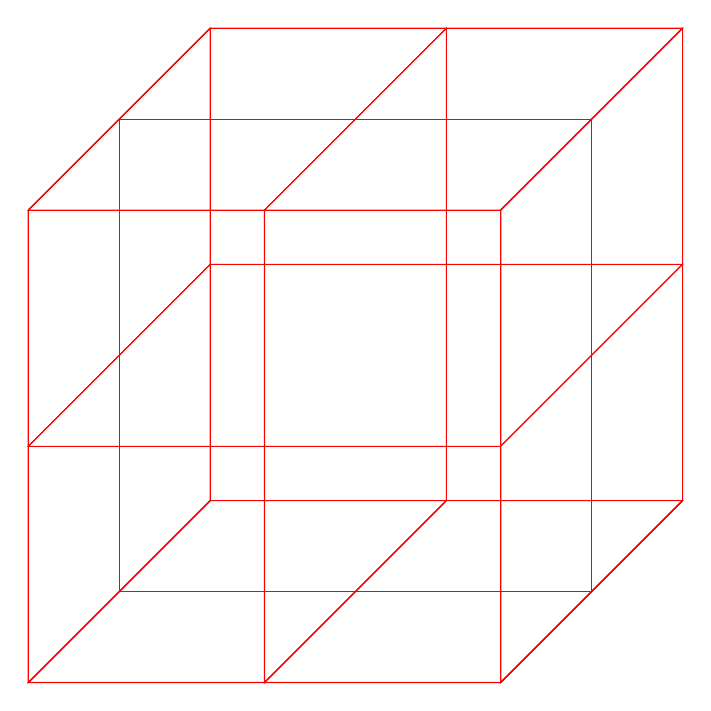
\begin{tikzpicture}[scale=1.5, transform shape]
    \begin{scope}[canvas is xy plane at z=0]
        \draw[red] (0,0) -- (4,0) -- (4,4) -- (0,4) -- cycle;
        \draw[red] (0,0) -- (0,4);
        \draw[red] (4,0) -- (4,4);
        \draw[red] (0,4) -- (4,4);
    \end{scope}
    
    \begin{scope}[canvas is yz plane at x=0]
        \draw[red] (0,0) -- (4,0) -- (4,4) -- (0,4) -- cycle;
        \draw[red] (0,0) -- (0,4);
        \draw[red] (4,0) -- (4,4);
        \draw[red] (0,4) -- (4,4);
    \end{scope}
    
    \begin{scope}[canvas is xz plane at y=0]
        \draw[red] (0,0) -- (4,0) -- (4,4) -- (0,4) -- cycle;
        \draw[red] (0,0) -- (0,4);
        \draw[red] (4,0) -- (4,4);
        \draw[red] (0,4) -- (4,4);
    \end{scope}
    
    \begin{scope}[canvas is xy plane at z=2]
        \draw[red] (0,0) -- (4,0) -- (4,4) -- (0,4) -- cycle;
        \draw[red] (0,0) -- (0,4);
        \draw[red] (4,0) -- (4,4);
        \draw[red] (0,4) -- (4,4);
    \end{scope}
    
    \begin{scope}[canvas is yz plane at x=2]
        \draw[red] (0,0) -- (4,0) -- (4,4) -- (0,4) -- cycle;
        \draw[red] (0,0) -- (0,4);
        \draw[red] (4,0) -- (4,4);
        \draw[red] (0,4) -- (4,4);
    \end{scope}
    
    \begin{scope}[canvas is xz plane at y=2]
        \draw[red] (0,0) -- (4,0) -- (4,4) -- (0,4) -- cycle;
        \draw[red] (0,0) -- (0,4);
        \draw[red] (4,0) -- (4,4);
        \draw[red] (0,4) -- (4,4);
    \end{scope}
    
    \begin{scope}[canvas is xy plane at z=4]
        \draw[red] (0,0) -- (4,0) -- (4,4) -- (0,4) -- cycle;
        \draw[red] (0,0) -- (0,4);
        \draw[red] (4,0) -- (4,4);
        \draw[red] (0,4) -- (4,4);
    \end{scope}
    
    \begin{scope}[canvas is yz plane at x=4]
        \draw[red] (0,0) -- (4,0) -- (4,4) -- (0,4) -- cycle;
        \draw[red] (0,0) -- (0,4);
        \draw[red] (4,0) -- (4,4);
        \draw[red] (0,4) -- (4,4);
    \end{scope}
    
    \begin{scope}[canvas is xz plane at y=4]
        \draw[red] (0,0) -- (4,0) -- (4,4) -- (0,4) -- cycle;
        \draw[red] (0,0) -- (0,4);
        \draw[red] (4,0) -- (4,4);
        \draw[red] (0,4) -- (4,4);
    \end{scope}
\end{tikzpicture}

\end{document}